%%%%%%%%%%%%%%%%%%%%%%%%%%%%%%%%%%%%%%%%%
% Template formal para se utilizar na equipe de propulsão e tecnologia aeroespacial (EPTA)
% LaTeX Template
% Version 1.0 (16/07/2019)
%
% This template was downloaded from:
%
% Original author:
% Peter Wilson (herries.press@earthlink.net) with modifications by:
% Vel (vel@latextemplates.com)
% Vel (feliperibeiro.ufu@gmail.com)
% Vel (mairaf_miranda@hotmail.com)
%
% License:
% CC BY-NC-SA 3.0 (http://creativecommons.org/licenses/by-nc-sa/3.0/)
%
% Conselhos para se lidar com este template:
% - Evitar alterar códigos referentes à formatação, com exceção de se copiar e colar
%          o código para exibição de imagens, tabelas e equações.
% - Procurar sempre manter as imagens utilizadas no documento em uma pasta dedicada,
%          de forma que, ao se referenciar a imagem, se referencie o caminho para 
%          ela, como feito com a "imagem_de_missao".
%
%
%%%%%%%%%%%%%%%%%%%%%%%%%%%%%%%%%%%%%%%%%

%----------------------------------------------------------------------------------------
%	Pacotes utilizados.(evitar mudar, se for necessária alguma mudança, comunicar gerencia)
%----------------------------------------------------------------------------------------

\documentclass[a4paper, 12pt,  oneside,a4paper,english,french,spanish,brazil]{book}     % Para folha A4, default 11pt tamanho
\usepackage[utf8]{inputenc}                                               % Acentos
\usepackage[brazil]{babel}                                                % Biblioteca para português
\usepackage{amssymb}                                                      % Biblioteca para símbolos
\usepackage{graphicx}                                                     % Biblioteca para figuras
\usepackage{tikz}                                                         % Pacote gráfico
\usepackage{amsmath}                                                      % Biblioteca para símbolos
\usepackage[T1]{fontenc}                                                  % encode para acentos 
\usepackage{fouriernc}                                                    % New Century Schoolbook font
\usepackage{xcolor}                                                       % Controle de cores
\usepackage[many]{tcolorbox}                                              % Controle de cores
\usepackage{amsthm}                                                       % Suporte matemático ams
\usepackage{physics}                                                      % Suporte em notações
\usepackage{gensymb}                                                      % Suporte em notação
\usepackage{amsfonts}                                                     % Suporte em fontes ams
\usepackage[left=1.00cm, right=1.00cm, top=3cm, bottom=2.50cm]{geometry}  % Parâmetros geométricos
\usepackage{caption}                                                      % Legenda para imagens
\usepackage{subcaption}                                                   % Legenda para figuras múltiplas
\usepackage{capt-of}                                                      % Suporte com legendas
\usepackage{float}                                                        % Suporte para maiores floats  
\usepackage[figurename=Fig.]{caption}                                     % Suporte 2 títulos legendas
\usepackage{tabularx}                                                     % suporte com tabelas
\usepackage{ragged2e}                                                     % suporte localização texto
\usepackage{mathrsfs}                                                     % Fontes para equações
\usepackage{makecell}                                                     % Formatação de tabelas
\usepackage{textpos}                                                      % Facilita posicionamento de forma absoluta
\usepackage[hyphens]{url}                                                 % Possibilita uso de hífen em links
\usepackage[makeroom]{cancel}                                             % Desconsidera limites para retas
\usepackage{empheq}                                                       % Possibilita emoldurar fórmulas
\usepackage[colorlinks=true,linkcolor=blue,urlcolor=blue,bookmarksopen=true, bookmarksnumbered, pdfencoding=auto]{hyperref}                                               % links clicáveis em PDF
\usepackage{fancyhdr}                                                     % Ajuda na criação de footers e headers
\usepackage{siunitx}                                                      % General suporte
\usepackage{enumitem}                                                     % Controle sobre layout
\usepackage{cancel}                                                       % Riscar coisas
\usepackage{bookmark}                                                     % Hiperlink em PDF
\usepackage{versions}                                                     % Devido às versões
\usepackage[pages=some,scale=1,angle=0,opacity=1]{background}             % Imagem de Background
\usetikzlibrary{decorations.pathmorphing}                                 % Permite utilização direta fonte abaixo
\usetikzlibrary{shapes.callouts,positioning}                              % Balões   
\usetikzlibrary{shapes.geometric,arrows,shadows}                          % flechas
\usepackage{frcursive}                                                    % Fonte cursiva
\usepackage{multirow}                                                     % Suporte tabelas

\setlength\parindent{3ex}                                                 % Parâmetro geométrico
\setlength{\parskip}{0.25em}                                              % Parâmetro geométrico
\setlength{\fboxsep}{10pt}                                                % Espaço ao redor dos quadros
\definecolor{zelena}{RGB}{0,100,0}                                        % Define cores em estruturas
\tcbuselibrary{theorems}                                                  % Cor nas caixas                           
\tcbuselibrary{breakable}                                                 % Particiona coisas
\pagestyle{fancy}  
\fancyhead[RO , RE]{\footnotesize 
	\begin{minipage}[b]{0.435\linewidth}\flushright\leftmark\end{minipage}}  % cabeçalho direito ímpar=título do capítulo
\fancyhead[LO , LE]{\footnotesize 	
	\begin{minipage}[b]{0.435\linewidth}\flushleft\rightmark\end{minipage}} % cabeçalho esquerdo = nome da seção
\fancyfoot[CE,CO]{\thepage}                                               % Nota de pé
\allowdisplaybreaks                                                       % Possibilita alguns comandos de controle
\setcellgapes{5pt}                                                        % Formatação de tabelas
\definecolor{eggshell}{rgb}{0.94, 0.92, 0.84}                             % Definição de cor 



\setlength\headheight{27.05003pt}
\renewcommand\headrule{\hrulefill
	\raisebox{10.1pt}[-10pt][-10pt]{\plogo}\hrulefill}                      % Headers
\newcommand{\plogo}{\fbox{  $EPTA$   }}                                   % sigla equipe 
\newcommand\BackImage[2][scale=1]{\BgThispage\backgroundsetup{
		contents={\includegraphics[#1]{#2}}}}                             % cria a função background
\newtcbox{\caixaeq}[1][]{nobeforeafter,math upper,tcbox raise base,enhanced,
	colframe=black!50!black,colback=eggshell!40!white,arc=4pt,	
	boxrule=1pt,drop fuzzy shadow,#1}                                     % Moldura para fórmulas

\DeclareMathOperator{\tg}{tg}                                             % Declara construção mat. 
\DeclareMathOperator{\cotg}{cotg}                                         % Declara construção mat.
%%%%%%%%%%%%%%%%%%%%%%%%%%%%%%%%%%%%%%%%%

\frontmatter
\date{}
%\thispagestyle{empty}
\date{\today}
\sloppy

%----------------------------------------------------------------------------------------
%    INÍCIO DO DOCUMENTO    (a partir daqui pode editar sem grandes complicações)
%----------------------------------------------------------------------------------------
\begin{document} 

%----------------------------------------------------------------------------------------
%	PÁGINA DE TÍTULO
%----------------------------------------------------------------------------------------

 \begin{titlepage} % Suprime cabeçalhos e notas na base da folha.

		\BackImage[scale = 1]{midia/epta_projeto_template}% imagem de background
	
	\begin{minipage}[h!]{0.37\textwidth}
		.%\textcolor{white}{.}% Para ocupar espaço (some times nothing is everything)
	\end{minipage}
	\begin{minipage}[h!]{0.6\textwidth}
	
		\centering % centraliza os textos na página
	
		\scshape % Usa formatação pequena 
	
		%------------------------------------------------
		%	Título
		%------------------------------------------------
	
		\rule{\textwidth}{1.6pt}\vspace*{-\baselineskip}\vspace*{2pt} % Linha horizontal grossa
		\rule{\textwidth}{0.4pt} % Linha horizontal fina
	
		\vspace{0.75\baselineskip} % espaço sobre o título
	
		{\LARGE Título do template base para relatórios da Equipe de Propulsão e Tecnologia Aeroespacial\\} % Título
	
		\vspace{0.75\baselineskip} % espaço abaixo do título
	
		\rule{\textwidth}{0.4pt}\vspace*{-\baselineskip}\vspace{3.2pt} % Linha horizontal fina
		\rule{\textwidth}{1.6pt} % Linha horizontal grossa
	
		\vspace{2\baselineskip} %espaço em branco abaixo do título
	
		%------------------------------------------------
		%	Subtítulo
		%------------------------------------------------
	
		Aqui coloca-se um subtítulo para descrever em linhas gerais o objetivo do texto. % descrição adicional (sub-título)
	
		\vspace*{3\baselineskip} % espaço abaixo do subtítulo
	
		%------------------------------------------------
		%	Autores(s)
		%------------------------------------------------
	
		Desenvolvido Por
	
		\vspace{0.5\baselineskip} % Espaço antes de autores
	
		{\scshape\Large Felipe J. O. Ribeiro \\ Maíra F. O. Miranda \\} % Lista de autores (ordem alfabética)
	
		\vspace{0.5\baselineskip} % Espaço após os autores
	
		\textit{Universidade Federal de \\ Uberlândia} % Entidades envolvidas
	
		\vspace{14.8\baselineskip} % Espaço (diminuir se houver mais autores)
	
		{\large Equipe de Propulsão e Tecnologia Aeroespacial} % equipe
		
		\vspace{0.3\baselineskip} % Espaço embaixo da logo
		
		Missão \_NOME DA MISSÂO\_ % Núcleo análogo
		
		\vspace{0.3\baselineskip} % Espaço embaixo da logo
		
		\today % Data de compilação
		
	\end{minipage}

\end{titlepage}

%----------------------------------------------------------------------------------------
%   Abstract...     (Um resumo do que será tratado em todo o texto)
%----------------------------------------------------------------------------------------
{
	\thispagestyle{empty}     % Sem numeração no abstract
	
	{\LARGE Abstract\\} % Abstract (grande)
	
	Neste local do texto coloca-se um breve resumo de tudo que irá constar no texto inteiro, para que os outros membros leiam e saibam exatamente do que o texto fala. Isso é necessário para que eles possam decidir se irão ler ou não este texto, e para facilitar a vida dos responsáveis por organizar a produção bibliográfica da equipe.
	
	Assim, será dado o exemplo agora, ou seja, direi tudo que será tratado dentro do texto. Primeiramente, será dado um breve resumo de formatação básica em latex, mudança de tamanho de texto, criação de capítulos, seções, subseções, etc... Funções em latex, disposição de parágrafos, comentários, espaçamento, automatizações da linguagem e criação de bullet points.
	
	Falar-se-á também sobre as motivações da criação deste template e suas finalidades. Se ensinará também como se cria urls clicáveis, também se explanando brevemente sobre nosso modelo de citações.
	
	Depois disso se fala sobre a formatação das equações, com diferentes formas de se manipular os números. Depois se fala de como importar imagens e sub-imagens, e como se utilizar o recurso das minipages para formatações mais ousadas de texto e imagens. Depois se mostra como utilizar a biblioteca Tikz para a criação de flowcharts e o que se pode adicionar nelas.
	
	Por fim se demonstra como criar tabelas dentro do latex, com exemplos bem interessantes, e se oferece uma ferramenta online, que alem de fazer o trem por você, pode ser uma boa ferramenta didática.
	
	Assim, a Equipe de propulsão e tecnologia aeroespacial agradece seu interesse em ler e aprender latex com este documento, mas na situação de dúvidas pode chamar o pessoal da gerencia. 
	
	Valeu.
	
	\vspace{1cm}
	{\large Palavras chave:} {\small Primeira palavra, Segunda palavra, terceira palavra, quarta palavra, quinta palavra, ...}

}
%----------------------------------------------------------------------------------------
%	Desenvolvimento...
%----------------------------------------------------------------------------------------

\tableofcontents          % Índice
\thispagestyle{empty}     % Sem numeração na página do índice
\listoffigures            % Lista de figuras 
\thispagestyle{empty}     % Sem numeração na página da lista de imagens
\mainmatter



\chapter{Introdução}%  <------------  Esse comando cria um capítulo

Olá caro integrante da Equipe de Propulsão e Tecnologia Aeroespacial que almeja escrever um texto relatório de circulação interna. Este documento está pronto para servir de base para sua empreitada. Aqui esta listado todo tipo de recurso para o pleno desenvolvimento desta tarefa de documentação que consideramos tão importante.

Aqui estão ferramentas para exibição de imagens, equações, tabelas, hiperlinks e texto nas mais diversas formatações. Assim, basta alterar o texto aqui contido de forma a tornar este documento um reflexo do trabalho desenvolvido pela equipe.

\section{Isso é uma sessão} %  <------------  Esse comando cria a sessão
É possível observar aqui a presença de uma sessão. O código referente a isso pode ser encontrado no texto fonte desse documento. Ela está referenciada com um "\%  <------------  Esse comando cria a sessão", nisso, o \% é o sinal para começar um comentário, assim "<------------  Esse comando cria a sessão" é ignorado pelo compilador.

Para começar um novo parágrafo, observe no código o espaço entre os textos, isso cria um novo parágrafo com edentação correta.

Nas páginas anteriores tem-se o título, altores e informações adicionais. Para mudar isto basta se procurar estes nomes nos códigos e mudar. Com as barras duplas pode-se por mais autores, se houverem mais de dois para este trabalho, dependendo da quantidade será necessário diminuir o tamanho do espaço após os autores.

Dessa forma basta agora que aprenda a importar os recursos gráficos, como segue no próximo tópico.

\subsection{Isso é uma sub sessão} % <---------------- Esse comando cria uma sub-sessão

Aqui se encontra um sub tópico do tópico. A formatação padrão da equipe só aceita até este nível de subdivisão, que provavelmente será suficiente às compulsões organizacionais mais violentas de você, singelo integrante da EPTA. \\
Usando barras duplas é possível começar um novo parágrafo, mas sem endentação padrão, ou seja, sem a margem estabelecida em template.  

Também para os designers de prontidão, é possível dar espaços arbitrários entre elementos do texto, usando o comando "vspace{1cm}" antecedido de uma barra. Neste caso, deu-se um espaço de 1 cm. (infelizmente houve quebra de página, sugiro usar o comando em outras linhas pra observar o espaço dado).

\vspace{1cm}

É possível observar também, no fundo da página, a numeração. Esta numeração aparece de forma automática e é atualizada também de forma automática, assim como capítulos no índice e a lista de imagens. As únicas páginas que não são contabilizadas são a capa e a página do índice.

Existe também o cabeçalho em cada página, mas ele só aparece em páginas que não são inícios de novos capítulos. E também não aparecem na capa e no índice. O texto livre colocado no código é transformado em texto corpo.

Há Muitos caracteres especiais que o latex permite. Tantas que nem posso listar (para mais exemplos, buscar na internet). Seguem as mais importantes:

\begin{itemize}
	\item Primeiramente é interessante observar como se fez esta lista de tópicos no código fonte. Começa-se um espaço do tipo "itemize" e se usa as funções "item" para criar os tópicos. 
	\item Algo interessante também é a função de criar textos em \textbf{negrito}. Isso pode ser visto também na documentação base, com a função "textbf".
	\item Para a utilização do  \textit{itálico} usa-se "textit", como amostrado no código fonte.
	\item Existem também comandos pra muitas formas de formatação de texto: \texttt{olá olá} , \LARGE olá olá , \normalsize olá olá, \scriptsize olá olá. \normalsize É interessante observar que ao usar uma dessas funções sem chaves, ele continua em vigor indefinidamente (estas funções em específico), é necessário chamar "normalsize" para voltar ao normal. 
\end{itemize}

\centering 
Também é possível centralizar o texto. Muito importante para fins estilísticos. Na equipe tal prática não é proibida nem incentivada. Uma questão de estilo.

Assim, tudo é centralizado, incluindo gráficos e tabelas.

Assim como as funções de formatação, esta continua em vigência de forma indefinida. Para liberar ao modo "normal", basta usar a função "flushleft".

\flushleft

Assim tem-se texto de volta ao normal.

\flushright 

Também é possível fazer o contrário, acumulando-se o texto a direita.

Nesse modo os textos acumulam-se todos à direita.

\flushleft                                                                % Joga tudo para a esquerda 
\setlength\parindent{3ex}                                                 % ajeita endentação
\setlength{\parskip}{0.25em}                                              % espaço paragrafo
% É necessário ajeitar essas coisas após mexer com a formatação.

Depois de mudar esse tipo de configuração é importante fazer tudo voltar ao normal. Usando as funções de levar tudo à esquerda e ajustar a margem e espaço entre parágrafos.

Assim temos novamente nossos parágrafos com espaçamento correto.

\subsection{Isso é outra sub sessão} 

Só para demonstrar a presença de duas dessas em um mesmo capítulo. Como não há muito o que falar, tenho que inventar qualquer texto para por aqui. Feito.

É bom mais um parágrafo para demonstrar o espaço de parágrafos funcionando bem também. Como pôde notar, o único início de parágrafo que não obedece a esse espaçamento é o primeiro de capítulos e seções. 

Apesar deste template não obedecer à ABNT, nosso foco é em deixar este documento bonito, profissional e prático. Um exemplo disto é o maior espaço por página, que possibilita figura e tabelas maiores e mais texto. Também, como estes documentos de circulação interna são pensados mais para serem lidos como PDF, espaço para encadernação é algo inútil. Assim podemos aproveitar bem o espaço das folhas e fazer o eptense leitor passar menos páginas.

Quando for o caso de transformar um destes documentos em ABNT para externalização de conteúdo, ou adequação de algum congresso, passar textos latex de um template a outro é muito simples. Nesse sentido, basta somente se lembrar de mudar as equações em que se utilizou funções criadas nesse template, como "caixaeq", mas nada que um "ctrl + f" não resolva.  

\section{Isso é outra seção}

Só para mostrar como ficam duas seções em um capítulo.

\subsection{Isso é mais uma outra subseção}

Só para mostrar como fica subseções em várias seções em um capítulo. Recomendo ver como fica bonito no índice.

\subsection{Índice interativo}

Algo interessante é que o índice é interativo, isto é, você pode clicar nos capítulos para ser levado a eles. Também é possível adicional url's clicáveis no pdf, como por exemplo: \url{https://en.wikipedia.org/wiki/Pikachu}

\subsection{Citações}

Para embasar bem o conhecimento desenvolvido pela equipe, citamos livros artigos e normas com bastante frequência. Para isso o Latex tem uma ferramente ótima, o bibfile. Nele você põe um banco de dados com todas as citações, e elas aparecem conforme você as chama dentro do texto. Isso permite que montemos um banco de dados com todas as citações já feitas pela equipe, basta que ao final de se redigir um texto, você encaminhe o bibfile final para o membro responsável que ele incluirá a citação no database do template, assim, com o tempo, esse data base ficará tão rico, que se tornará raro a necessidade de inclusão de novas referencias.

Para se citar uma referencia da bibfile, basta usar o comando "cite", e o resultado é: \cite{CavaliniJunior2015}

\chapter{Equações matemáticas}


Muito importante também nos relatórios da EPTA são as equações. Seja em situações de dimensionamento ou embasamento teórico. Assim, este template oferece opções muito interessantes para embarcar os desenvolvimentos matemáticos do seu projeto. 

Primeiramente, é possível colocar uma equação no meio de um parágrafo de texto, com "\$". Como por exemplo "\$ frac\{1\}\{2\}\$" resulta em "$\frac{1}{2}$". É interessante notar que quando se quer por um simbolo que é utilizado em funções de programação, basta colocar uma barra antes. Isso é especialmente útil para representar grandezas de dentro da função no texto, como $L.W_{minimo}^2$. Ou seja, as grandezas vistas na equação podem estar todas dentro do texto, o que facilita explicações e referencias a coisas específicas de dentro das equações.

Adiante exemplificaremos uma forma de demonstrar equações:

\begin{equation}\label{equacao1}
	\caixaeq{                            % as duas linhas abaixo estão dentro desta função (criar caixa)
		P=\frac{U}{I}                    % equação
		\quad                            % dá o espaço entre equação e texto
		\text{\footnotesize(Oloco, posso por parenteses ao lado da equação)}    % função text cria texto dentro de ambiente de equação
	} 
\end{equation}

Esse formato é guardado para equações importantes, como fórmulas de onde parte um desenvolvimento algébrico, ou resultados finais.

Outra forma de representação é a mais simples:

\begin{equation}\label{equacao2}
	\frac{\partial Q}{\partial t} = Q^\prime
\end{equation}

Latex é incrível para fazer equações. A praticidade permite o desenvolvimento de equações excepcionalmente grandes, e quando se pega o jeito, torna-se mais simples fazer isso em latex que no word. Como pode-se ver na Eq.\ref{equacao3}:
\begin{equation}\label{equacao3}
	\frac{\partial \overline{T}}{\partial t} +\frac{\partial{}}{\partial{x}} \left(\overline{T^\prime  u^\prime}\right) + \frac{\partial{}}{\partial{x}}\left(\overline{u} \ \overline{T}\right)     + 
	\frac{\partial{}}{\partial{y}} \left(\overline{T^\prime v^\prime}\right) + \frac{\partial{}}{\partial{x}}\left(\overline{v} \ \overline{T}\right) 
	=
	{\frac{\partial{}}{\partial{x}}} \left(\alpha {\frac{\partial{\overline{T}}}{\partial{x}}} \right) +
	{\frac{\partial{}}{\partial{y}}} \left(\alpha {\frac{\partial{\overline{T}}}{\partial{y}}} \right) .
\end{equation}

Uma boa funcionalidade do latex é a facilidade de se referenciar os elementos do texto. Se observar com atenção a função que deu origem a esta equação, observará uma componente "label" dentro, que serve para se referenciar esta equação dentro do texto. Quando for necessário se referenciar ela, basta usar a função "ref", resultando em "\ref{equacao1}". Neste template decidiu-se a seguinte formatação para referencias às equações: "Eq.\ref{equacao1}". O nome utilizado nas Labels é completamente arbitrário. Ele só precisa ser única (não se pode ter duas ou mais equações com a mesma label).

Quanto à se acostumar com o código, acredito que a melhor forma de se aprender é observar exemplos, assim, disponibilizo abaixo vários exemplos de equações, na internet também há documentação para tudo que se possa imaginar: 

\begin{equation}
T_m(x) = \frac{\int u(y) T(x , y) dy}{\int u(y)  dy} .
\end{equation}

Para equações maiores é possível quebrá-la em partes, mas é aconselhável se utilizar os comandos na equação a seguir, para mantar-se centralizada e bem distribuída a equação:

\begin{center}
\begin{equation}
	\begin{split}
	\frac{\partial ( \overline{ T^\ast + T_w } ) }{\partial t} +
	\frac{\partial{}}{\partial{x}} \left(\overline{T_w^{\prime} u^{\prime}}\right) +\frac{\partial{}}{\partial{x}} \left(\overline{{T^{\ast}}^{\prime} u^{\prime}}\right)
	+\frac{\partial{}}{\partial{x}}\left(\overline{u} \ \overline{T^{\ast}}\right)+ 
	\frac{\partial{}}{\partial{x}}\left(\overline{u} \ \overline{T_w}\right)+ 
	\\
	\frac{\partial{}}{\partial{y}} \left(\overline{{T^{\ast}}^{\prime} v^{\prime}}\right)+
	\frac{\partial{}}{\partial{y}} \left(\overline{T_w^\prime v^\prime}\right) + \frac{\partial{}}{\partial{y}}\left(\overline{v} \ \overline{T^\ast}\right) +
	\frac{\partial{}}{\partial{y}}\left(\overline{v} \ \overline{T_w}\right) 
	= 
	\\
	{\frac{\partial{}}{\partial{x}}} \left(\alpha {\frac{\partial{\overline{(T^\ast + T_w)}}}{\partial{x}}} \right) +
	{\frac{\partial{}}{\partial{y}}} \left(\alpha {\frac{\partial{\overline{(T^\ast + T_w)}}}{\partial{y}}} \right) .
	\end{split}
\end{equation}
\end{center}

Também é possível mudar a cor de elementos dentro da equação, e isso pode ter consequências muito positivas na explicação de desenvolvimentos algébricos:

\begin{center}
\begin{equation}
	\begin{split}
	\color{red}\frac{\partial ( \overline{ T^\ast + T_w } ) }{\partial t} \color{black} +
	\frac{\partial{}}{\partial{x}} \left(\overline{ \color{red}T_w^{\prime} \color{black} u^{\prime}}\right) +
	\color{red}\frac{\partial{}}{\partial{x}} \left(\overline{{T^{\ast}}^{\prime} u^{\prime}}\right)+ \color{black}
	\color{red} \frac{\partial{}}{\partial{x}}\left(\overline{u} \ \overline{T^{\ast}}\right) \color{black}+ 
	\frac{\partial{}}{\partial{x}}\left(\overline{u} \ \overline{T_w}\right)+ 
	\\
	\frac{\partial{}}{\partial{y}} \left(\overline{{T^{\ast}}^{\prime} v^{\prime}}\right)+
	\frac{\partial{}}{\partial{y}} \left(\overline{\color{red}T_w^\prime \color{black} v^\prime}\right) + \frac{\partial{}}{\partial{y}}\left(\color{red}\overline{v} \color{black} \ \overline{T^\ast}\right) +
	\frac{\partial{}}{\partial{y}}\left(\color{red}\overline{v}\color{black} \ \overline{T_w}\right) 
	= 
	\\
	\color{red}{\frac{\partial{}}{\partial{x}}} \left(\alpha {\frac{\partial{\overline{(T^\ast + T_w)}}}{\partial{x}}} \right) \color{black}+
	{\frac{\partial{}}{\partial{y}}} \left(\alpha {\frac{\partial{\overline{(T^\ast + \color{red} T_w \color{black})}}}{\partial{y}}} \right) .
	\end{split}
\end{equation}
\end{center}

Ao se acostumar com a linguagem, fazer equações muito complexas pode ser mais simples do que se pensa:

\begin{equation}
	{\frac{\partial{}}{\partial{\tilde{y}}}} \left( \left( \frac{Re_\tau}{Pr}   
	- \frac{{L}^2 Re_\tau ^3}{Pr_t}\frac{\partial \tilde{\overline{u}}}{\partial \tilde{y}} \right) \frac{\partial \tilde{\overline{T^\ast}}}{\partial \tilde{y}} \right)
	= 
	\frac{\tilde{\overline{u}}}{\tilde{u_m}}.
\end{equation}

Também é possível se utilizar funções para equações, um caso interessante é o da função "cases", que possibilita:

\begin{equation}
	\label{ola}
	\text{Propriedades}=
	\begin{cases}
		\overline{f}({x})=\frac{1}{t_f - t_i} \int_{t_i}^{t_f} f({x} , t) dt.      & \quad  \\
		f({x} , t) = \overline{f}({x}) + f^\prime ({x} ,t) . & \quad   \\
		\overline{f^\prime ({x} ,t)} = 0 . & \quad   \\
		\overline{\overline{f({x})}} = \overline{f({x})} . & \quad   \\
		\overline{f^\prime ({x} ,t)\overline{f({x})}} = 0 .& \quad   \\
		\overline{f^\prime ({x} ,t)g^\prime ({x} ,t)} \neq 0 . & \quad   \\
		\overline{  \overline{g({x})} \ \overline{f({x})}  } = {\overline{g({x})}} \ {\overline{f({x})}} . & \quad   \\
	\end{cases}
\end{equation}

\section{Mais uma seção, pq não?}

Para esta última seção guardamos o mais interessante:

 \rotatebox{90}{$ \frac{1}{2}$} 

O próximo exemplo permite encadear várias equações uma atrás da outra, separadas por barra dupla. Observa-se também dois métodos de se escrever o "seno". Neste template achamos cômodo usar o padrão internacional "sin":
\begin{eqnarray}
	\frac{1}{n} \sin x & = & \mathrm{?} \\
	\frac{1}{\cancel{n}} \mathrm{si}\cancel{\mathrm{n}} ~x & = & \mathrm{?} \\
	\mathrm{six} & = & 6 \quad \text{(só leio verdades)}
\end{eqnarray}

Utilizando a biblioteca Tikx é possível se fazer também loucuras, como desenhar um triangulo a partir de código no latex, como no exemplo "onde está o $x$?", abaixo:

\begin{figure}[h!]
	\centering
\begin{tikzpicture} 
\draw (0,0) -- (4,0) node[midway,below] {4 cm}
-- (4,3) node[midway,right] {3 cm}
-- (0,0) node[midway,left,circle,draw=blue,decorate,decoration={random steps,segment length=1pt,amplitude=0.5pt}]{$x$}
-- (4,0) rectangle (3.7,0.3)
-- cycle;
\draw (0.4,0) arc (0:30:0.5);
\draw (4,2.6) arc (270:226:0.5);
\draw (1,2.1) node []{\color{blue}\fontfamily{frc}\selectfont{Aqui está !!}};
\end{tikzpicture}
\end{figure}

Dessa forma, essa ferramenta pode ser utilizada para, virtualmente, se fazer qualquer coisa.

Mas a utilização do tikz é opcional. Muito mais prático é criar imagens em programas como photoshop ou paint e importar com a ferramente de amostragem de imagens. Mas como fazer isso ?



\chapter{Trabalhando com imagens}



Para trabalhar com imagens, basta adicionar um arquivo na pasta onde se encontra o código fonte deste documento e chamá-la com a função dedicada para isso:


\begin{figure}[h!]
	\centering
	
\includegraphics[trim = {0cm 0cm 0cm 0cm}, clip , angle=0, scale=0.30]{midia/exemplo}
	\caption{"todos os relatórios na epta são feitos em LaTex".}
	\label{pika1}
\end{figure}

Também é possível por várias figuras em uma figura. Se isso não fez muito sentido, observar exemplo a seguir:

\begin{figure}[h!]
	\centering
	\begin{subfigure}[b]{0.3\textwidth}
		\centering
		
\includegraphics[width=\textwidth]{midia/exemplo}
		\caption{estou na esquerda}
		\label{pika2}
	\end{subfigure}
	\hfill
	\begin{subfigure}[b]{0.3\textwidth}
		\centering
		
\includegraphics[width=\textwidth]{midia/exemplo}
		\caption{estou no centro}
		\label{pika3}
	\end{subfigure}
	\hfill
	\begin{subfigure}[b]{0.3\textwidth}
		\centering
		
\includegraphics[width=\textwidth]{midia/exemplo}
		\caption{estou na direita}
		\label{pika4}
	\end{subfigure}
	\caption{Três pikashus, entendeu?}
	\label{pika5}
\end{figure}

Assim, é possível adicionar imagens com um vínculo lógico entre elas. E elas todas são igualmente muito bem referenciáveis. Assim como com as equações, neste template escolhemos referenciar imagens com "Fig.\ref{pika4}", ou "Fig.\ref{pika5}". A forma de referencia é parecida com as de equações.

\section{Minipage, o que é?}

Há também uma forma de se dispor elementos lado a lado se a necessidade de subfigures, e, o mais interessante, é que é possível por texto ao lado de imagens com esse método. Basta utilizar a função "minipage". 	

\begin{figure}[ht]
	\begin{minipage}[b]{0.45\linewidth}
		\centering
		
\includegraphics[trim = {0cm 0cm 0cm 3cm} , clip , width=\textwidth]{midia/exemplo}
		\caption{Estou a esquerda, mas sou uma figura normal.}
		\label{pika88}
	\end{minipage}
	\hspace{0.5cm}
	\begin{minipage}[b]{0.45\linewidth}
		\centering
		
\includegraphics[trim = {0cm 0cm 0cm 3cm} , clip  , width=\textwidth]{midia/exemplo}
		\caption{Estou a direita, mas sou uma figura normal.}
		\label{pika99}
	\end{minipage}
\end{figure}

Agora, vou compartilhar um exemplo. Colocando-se texto e equações ao lado de uma imagem. É importante salientar que além de textos e imagens, qualquer elemento gráfico pode ser colocado em uma "minipage". Segue um exemplo muito instrutivo:

\begin{figure}[ht]
	\begin{minipage}[b]{0.45\linewidth}
		O flamingo é uma ave pertencente à família Phoenicopteridae da ordem Phoenicopteriformes. Anteriormente pertencia a ordem Ciconiiformes. Tradicionalmente todas as espécies eram incluídas no género Phoenicopteruss, mas actualmente o flamingo-andino e o flamingo-de-james são considerados um gênero à parte, Phoenicoparrus, por causa de certas diferenças no bico, e o flamingo-pequeno também foi incluído no seu próprio género, Phoeniconaias.
		\begin{equation}
		\text{cor}_{rosa} + \text{ave} = flamingo
		\end{equation}
		\vspace{0.5cm}
	\end{minipage}
	\hspace{0.5cm}
	\begin{minipage}[b]{0.45\linewidth}
		\centering
		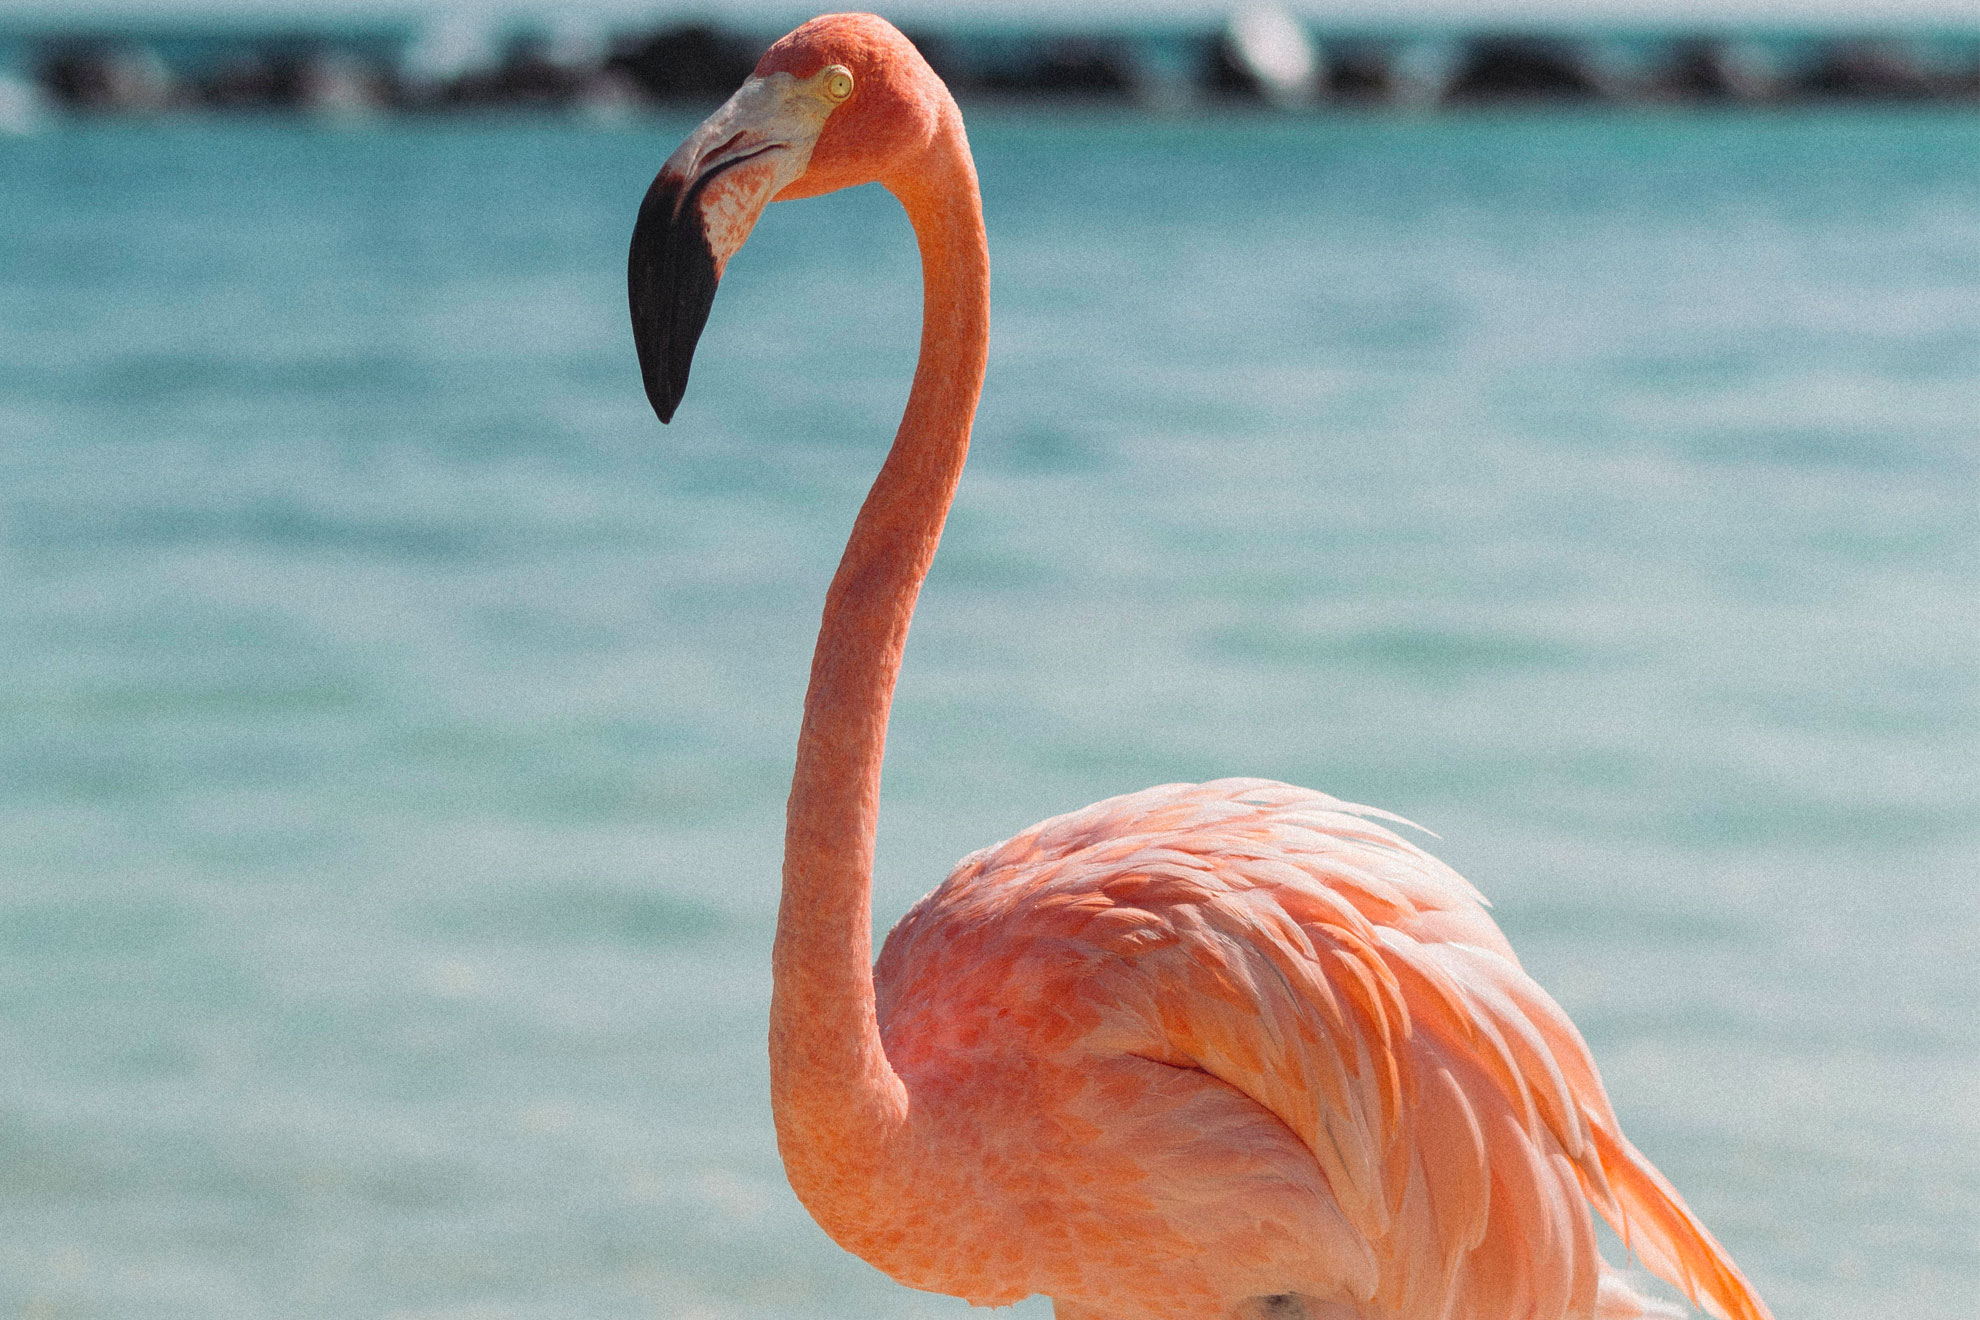
\includegraphics[trim = {10cm 0cm 10cm 0cm}, clip , width=\textwidth]{midia/exemplo2}
		\caption{Ave rosa, AKA flamingo.}
		\label{pika11}
	\end{minipage}
\end{figure}

Se você observar o texto instrutivo ao lado da imagem acima, observará que "vspace" está sendo usado para localizar o texto corretamente ao lado da imagem.

A utilização destas ferramentas todas são opcionais e algo que tem dependência completamente estilística. Deixar textos acadêmicos bonitos é parte do trabalho de um cientista, pois de nada adianta criar muita informação se você não consegue passar isso adiante de forma efetiva. 

\section{Criando flowcharts com tecnicas de tikz (obs: vejo o que ocorre com títulos de capítulos muito muito grandes...)}

Como se já não fosse o bastante, também é possível se criar diagramas com a biblioteca tikz. Apesar de ser algo um tanto avançado, e haver softwares que fazem isso de forma muito simples, fica a recomendação da utilização do pacote tikz, por proporcionar homogeneidade e controle estilístico. Mas ressalto que é uma opção sua utilização, visto que é perfeitamente possível, se criar estes diagramas com programas externos, salvando-se eles como PDF ou png e importando eles como mostrado anteriormente. Mas fica a escolha de se fazer isso inteiramente dentro da plataforma latex.


%Criando os formatos:
\tikzstyle{rect} = [draw, rectangle,fill = gray!20, text width=6em, text centered, minimum height = 2em ]
\tikzstyle{elli} = [draw, ellipse,fill=white!20,minimum height=2em]
\tikzstyle{circ} = [draw, circle,fill=white!20, minimum width=8pt,inner sep=10pt]
\tikzstyle{diam} = [draw, diamond,fill=white!20,text width=6em, text badly centered, inner sep=0pt]
\tikzstyle{line} = [draw, -latex']

%Criando o flowshart:
\begin{figure}[h]
	\begin{center}
		\begin{tikzpicture}[node distance = 1.5cm, auto]
		\node[rect, rounded corners](step1) { necessidade de um flowchart};
		\node[rect,rounded corners , right of=step1, node distance=4.5cm] (step2) {Esquema de flowchart criado};
		\node[rect, right of=step2, node distance=4.5cm] (step3) {$P^\prime = \frac{\vec{U_m}}{\partial t}$};
		\node[rect, right of=step3, node distance=4.5cm] (step4){
\includegraphics[trim = {0cm 0cm 0cm 0cm}, clip , width=\textwidth]{midia/exemplo}};
		\node[rect, rounded corners, below of=step4, node distance=4.5cm](step5){Flowchart final};
		
		\path[line](step1) -- node [above, text width=4em] {Organização das ideias.} node [below, text width=4em] { É possível citar Eq.\ref{equacao2}} (step2);
		
		\path[line](step2) -- node [above, text width=4em] {Escrita do código} node (line2) [below, text width=4em] {Imagens e equaçõe} (step3);
		
		\path[line](step3) -- node [above, text width=4em] {Dá de por imagens?} node [below, text width=4em] {} (step4);
		
		\path[line](step4) -- node [left, text width=5em] {Ok, tudo pronto} (step5);
		
		\path[line](step5) -| node [right, near end, text width=6em] {Não, vishe, refaz} (line2);
		
		\path[line](step5) -| node [right, near end, text width=6em] {Sim, de acordo, fechouu} node [below, near start, text width=12em] {Gostei do meu flowchart?} (step1);
		\end{tikzpicture}
	\end{center}
	\caption{Processo de criação de um flowchart (mais ou menos).}
\end{figure}

Assim, observando-se o código, é possível editar este flowchart para a maioria das aplicações. Mas, se for do interesse mais detalhes, recomendo estudar a documentação da biblioteca Tikz. Ela está disponível de graça na internet. (\url{http://www.texample.net/tikz/}) É incrível o que se pode fazer com essa biblioteca.



\chapter{Trabalhando com tabelas}

Outro recurso importante é a habilidade de se fazer tabelas. Muitas vezes, para se ilustrar dados, nada mais esclarecedor que uma tabela. Tais construções também são úteis para listagens como de preço, massa ou altura no foguete. 

Segue o exemplo de uma tabela padrão latex: 


\begin{table}[h!]
	\centering
	\begin{tabular}{|llll|l}
		\cline{1-4}
		\multicolumn{1}{|l|}{Peça} & \multicolumn{1}{l|}{Preço} & \multicolumn{1}{l|}{Massa} & Espaço  ocupado &  \\ \cline{1-4}
		1                          & 10,00 R\$                  & 40 g                       & 30 cm           &  \\
		2                          & 25,00 R\$                  & 20 g                       & 20 cm           &  \\
		3                          & 43,00 R\$                  & 57 g                       & 50 cm           &  \\ \cline{1-4}
	\end{tabular}
	\caption{tabela para fins de exemplo.}
\end{table}


Recomendamos aprender a sintaxe da criação de tabelas, mas oferecemos também ferramentas que auxiliem. Nesse site há um programa online que cria o código para você:
\url{https://www.tablesgenerator.com/}

Porém, aprender a linguagem permite que crie tabelas mais bonitas e completas:

\begin{table}[h!]
	\centering
	\begin{tabular}{|c|c|c|c|c|c|}
		\hline
		\multirow{3}{*}{
\includegraphics[trim = {0cm 0cm 0cm 0cm}, clip , scale = 0.03]{midia/exemplo}} & \multicolumn{2}{c|}{Algo B} & %
		\multicolumn{2}{c|}{Algo C} & \multirow{3}{*}{
\includegraphics[trim = {0cm 0cm 0cm 0cm}, clip , scale = 0.03]{midia/exemplo}}\\
		\cline{2-5}
		& \multicolumn{2}{c|}{Valor} & \multicolumn{2}{c|}{Valor} & \\
		\cline{2-5}
		& B1 & B2 & C1 & C2 & \\
		\hline
		& & & & & \\
		\hline
		& & & & & \\
		\hline
		% etc. ...
	\end{tabular}
	\caption{Outra tabela exemplo.}
\end{table}

É possível se inserir todo tipo de elemento gráfico nestas tabelas, abrindo margem para muita liberdade criativa.

Fora a metodologia recomendada, também são possíveis soluções menos recomendadas. Uma delas é se criar a tabela em outro software, vulgo excel, por exemplo, e salvá-la como pdf. Depois basta importar ela da mesma forma que importamos todos os pikachus até o momento. O latex trata o pdf como uma imagem, mas suas propriedades de vetorização dos gráficos são mantidas. 
Dessa forma recomenda-se fortemente sempre se utilizar Pdf's para guardar qualquer recurso gráfico.

%----------------------------------------------------------------------------------------
% Bibliografia.
%----------------------------------------------------------------------------------------


\bibliographystyle{unsrt}
\bibliography{bibfile}



\end{document}
